%
% The first command in your LaTeX source must be the \documentclass command.
\documentclass[sigconf]{acmart}
\settopmatter{printacmref=false}
\usepackage[T1]{fontenc}
%\usepackage{lmodern}
\usepackage{mathtools}
%
% defining the \BibTeX command - from Oren Patashnik's original BibTeX documentation.
\def\BibTeX{{\rm B\kern-.05em{\sc i\kern-.025em b}\kern-.08emT\kern-.1667em\lower.7ex\hbox{E}\kern-.125emX}}
    
% Rights management information. 
% This information is sent to you when you complete the rights form.
% These commands have SAMPLE values in them; it is your responsibility as an author to replace
% the commands and values with those provided to you when you complete the rights form.
%
% These commands are for a PROCEEDINGS abstract or paper.
\copyrightyear{2018}
\acmYear{2018}
\setcopyright{acmlicensed}
\acmConference[RecSys '19]{Recomme '18: ACM Symposium on Neural Gaze Detection}{September 16--20, 2019}{Copenhagen, Denmark}
\acmBooktitle{RecSys '19: ACM Conference on Neural Gaze Detection, June 03--05, 2018, Woodstock, NY}
\acmPrice{15.00}
\acmDOI{10.1145/1122445.1122456}
\acmISBN{978-1-4503-9999-9/18/06}

%
% These commands are for a JOURNAL article.
%\setcopyright{acmcopyright}
%\acmJournal{TOG}
%\acmYear{2018}\acmVolume{37}\acmNumber{4}\acmArticle{111}\acmMonth{8}
%\acmDOI{10.1145/1122445.1122456}

%
% Submission ID. 
% Use this when submitting an article to a sponsored event. You'll receive a unique submission ID from the organizers
% of the event, and this ID should be used as the parameter to this command.
%\acmSubmissionID{123-A56-BU3}

%
% The majority of ACM publications use numbered citations and references. If you are preparing content for an event
% sponsored by ACM SIGGRAPH, you must use the "author year" style of citations and references. Uncommenting
% the next command will enable that style.
%\citestyle{acmauthoryear}

%
% end of the preamble, start of the body of the document source.
\begin{document}

%
% The "title" command has an optional parameter, allowing the author to define a "short title" to be used in page headers.
\title{The Ex-Ante View of RS Design}
%
% By default, the full list of authors will be used in the page headers. Often, this list is too long, and will overlap
% other information printed in the page headers. This command allows the author to define a more concise list
% of authors' names for this purpose.

%
% The abstract is a short summary of the work to be presented in the article.
\begin{abstract}
Recommender systems (RS) are traditionally deployed in environments where users are uncertain about their preferences and thus face a problem of choice under uncertainty, but most popular design approaches ignore this fact. We argue that predicting and modeling consumer choice in these contexts can improve the usefulness of RS and reframe the RS problem as providing useful information to help reduce user uncertainty as opposed to simply predicting user preferences. We show how this insight can be utilized to design RS that mitigate the negative consequences of RS such as filter bubble and user homogenization effects as well as better understand the role that RS play in contributing to these phenomena.
\end{abstract}

%
% The code below is generated by the tool at http://dl.acm.org/ccs.cfm.
% Please copy and paste the code instead of the example below.
%

%
% Keywords. The author(s) should pick words that accurately describe the work being
% presented. Separate the keywords with commas.
\keywords{Recommender Systems, Beliefs, Decision Theory, Filter Bubbles}

%
% This command processes the author and affiliation and title information and builds
% the first part of the formatted document.
\maketitle

\section{Introduction}

Recommender Systems (RS) have been widely deployed in online platforms such as Netflix, Amazon, and YouTube. On these platforms the combination of the fact that most goods are experience goods and that the number of choices available to users is incredibly large results in users not knowing their true preference ordering over all of the items. For instance, on Netflix there are thousands of movies, on Amazon there are millions of products, and on YouTube there are billions of videos. As a result, RS have been useful in helping users make decisions on these platforms because they provide users with information to help them make their choices under uncertainty. 
\par
However, while acknowledging that this is why RS are useful, most of the literature on RS ignores this user uncertainty and takes what we call an \textit{ex-post} viewpoint to preferences, focusing on the reported utility of users after they consume the item or inferring them via behavioral data \cite{adomavicius2005toward, zhao2018interpreting}. The RS problem traditionally is cast as solving the following prediction problem:
\begin{align*}
\arg\max\limits_{x \in A} u(x)
\end{align*}
\noindent where $A$ is the set of possible items and $u(x)$ represents the utility a user gets to consume good $x$. Recently there has been a move away from metrics focused on maximizing the accuracy of this prediction problem and towards optimizing for metrics such as serendipity or discoverability \cite{mcnee2006being, vargas2011rank} due to  the realization that accurate recommendations may not be the most useful recommendations for users. Furthermore, deployed RS have come under scrutiny for leading to ``filter bubbles" \cite{pariser2011filter} where users consume a less diverse set of content over time as well as increased homogenization amongst users \cite{chaney2018algorithmic, hosanagar2013will}.
\par
In this paper we want to put forward the argument that one approach to overcoming these problems is to make understanding how users choose which goods to consume a first-order consideration when designing RS. In particular, we differentiate between the previous \textit{ex-post} interpretation of the RS problem and what we define as the \textit{ex-ante} viewpoint. Unlike the ex-post viewpoint taken in the traditional prediction problem, the ex-ante viewpoint simply states that users face uncertainty and so maximize their expected utility as is defined in economic decision theory under uncertainty \citep[see e.g.][]{mas1995microeconomic}:
\begin{align*}
\arg\max\limits_{x \in A} \mathbb{E}[u(x)]
\end{align*}
Fundamentally, the move away from accuracy towards alternative metrics as well as tensions that have arisen from increased user homogenization and filter bubbles come from the \textit{choices} that users make. This shift from thinking about true preferences after all uncertainty is resolved (the ex-post view) to user decisions under uncertainty (the ex-ante view) can serve as a theoretical tool to better understand what recommendations are useful for users as well as understanding what of the documented perverse effects of RS come from recommendation per-se and what effects come from inherent uncertainty in user decision-making.
\section{The Value of Understanding User Beliefs in RS}

In this section we illustrate the differences between the ex-post and ex-ante view and show how it is useful for thinking about the design of RS. Our first point is trivial to state - since users do not know the true consumption values of the items, without any further information they may make sub-optimal consumption decisions. Consider the following stylized example. The choice set of the individual is $\Omega= \{x_1, x_2, x_3 \}$ and the ex-post utility values are given by
$u(x_1) = 1$, $u(x_2) = 2$, $u(x_3) = 3$. 
\par
However, when users are making decisions they have unobservable \textit{beliefs} about the ex-post utility value of the items and make decisions given these beliefs. If users had more information then their beliefs would converge to the ex-post utility values but, generally, users do not have enough information and so have beliefs over the space of possible ex-post utility values. In this example we suppose these beliefs are simple so that users view each good as simple lotteries: for $n=1,2,3$, $u(x_n) = n + \varepsilon_n$, $\varepsilon_1 \sim \mathcal N (2, 1)$, $\varepsilon_2 \sim \mathcal N (0, 1)$, $\varepsilon_3 \sim \mathcal N (-5, 1)$.
\par
In this example, after uncertainty is unresolved, the user ought to consume $x_3$, but an expected utility maximizing consumer (without further information) would consume $x_1$.\footnote{Note that here we ignore an important component of decision-making under uncertainty from decision theory, risk preferences, and suppose users are risk-neutral. A \textit{risk-averse} user may choose to consume a good with lower expected payoff but lower ex-ante variance compared to another good. While risk-aversion is an important component of decision-making and important in the context of RS when considering choices under uncertainty, it is not our main focus here.}
\par
This observation, while seemingly trivial, has important implications. The fact that the user would choose $C$ over $A$ reveals that $C$ prefers $A$ and allows us to get some information about a user's beliefs. Why are user beliefs important objects for designers of RS to understand and utilize?
\par
The first is that they are useful for understanding how users interact and get value from RS. In particular, users use RS to get \textit{information} about the set of items and update their beliefs about the value of the items. For instance, in the example, a RS could recommend to a user $x_3$ over $x_2$ and $x_1$ and that user will use this to update her beliefs about $x_3$. It is an empirical question that we leave for future work precisely how and to what extent users update their beliefs from recommendation and what factors of RS deisgn influence this.\footnote{There has been some work in this direction in understanding when recommendations are persuasive \cite{cremonesi2012investigating, gretzel2006persuasion} as well as the effect of their delivery on effectiveness \cite{murphy2014recommendation}.}
\par
Better understanding user beliefs is important for improving the performance of RS that optimize for metrics that move away from accuracy such as serendipity \cite{kotkov2016survey}. Serendipity-based RS attempt to provide recommendations that ``have the quality of being both unexpected and useful" \cite{maksai2015predicting} but it is hard to know what items are both unexpected and useful \cite{kotkov2016survey}. Understanding \textit{why} a user has not consumed a good depends on the beliefs that the user has and this is important for designing serendipitious recommendations. For instance, in the example, the user does not consume $x_3$ because she believes that the good has the potential to be catastrophically bad but, given more information, she would prefer to consume it over $x_1$ and $x_2$. It is possible that the ex-post and ex-ante utility of $x_3$ could be at best as good as the other two. The user may have an alternative with a known value -- say going for a walk around the neighborhood -- which she could always prefer to watching a given movie that has uncertain value but that the consumer thinks is always lower than the value of the walk.
\footnote{An additional reason this could be useful is if one considers a risk-averse individual, then it may be that a user has not consumed an item because she has a high perceived variance for the item but high expected quality.}
As a result, understanding the beliefs of users helps us understand why users have not consumed certain items and, in particular, which items a user may find useful given more information about it. This poses an important problem: designing systems that elicit not only ex-post valuations but also ex-ante beliefs about valuations, as only by knowing these can RS be effective in steering users' choices.
\par
Understanding the choices that individuals will make as well as what they will end up liking are complementary problems but require different viewpoints. \cite{jiang2014choice, saavedra2016choice} argue that choice-based approaches alone can help in designing better RS, though they argue that for these approaches because they do a better job at providing more accurate recommendations. We argue that the two problems should be considered separately -- though they may interact in interesting and useful ways.\footnote{In particular, some of the results from \cite{jiang2014choice, saavedra2016choice} may be driven by the fact that user choice embeds ratings information that may not have been observed by the recommender but is observed by the user. For instance, on Netflix I may have seen every episode of Friends when it was on TV which influences the consumption choices that I make. Alternatively, my friends can be a source of information that affect beliefs and choices. Netflix cannot observe neither of these data.} 
\par
RS are designed to give users \textit{information} that is useful to help them make decisions. On the one hand, predicting what are a user's ex-post preferences is useful to know what items the user would like to consume. On the other hand, predicting what items a user will actually consume (without recommendation) can help reason about what information may actually be useful to give her. Furthermore, in designing RS to avoid filter bubble and homogenization effects, having accurate choice predictions allows mitigating such adverse effects to become a first-order component of design. In particular, by predicting both choice and ratings, RS can provide information to users that leads them to useful goods but prevents them from falling into a filter bubble. 
\par
Solving this choice prediction problem requires data on the choices that individuals make and the sets that they choose them from as opposed to the traditional ratings or behavioral data that is collected. In the example given previously the fact that the consumer chooses $x_1$ from the set $\{x_1, x_2, x_3 \}$ would be the data that is useful for the choice prediction problem.

\section{Consumer Learning and Filter Bubbles}\label{sec:consumer_learning}
In this section we further show that differentiating between the ex-ante and ex-post view allows us to not only design better RS but also better understand their consequences. To do so, we study a simple model where users have beliefs about how good each item is and can learn their valuation over the items by consuming them. However, this learning process has spill-overs to their beliefs about other similar items which influences their future consumption choices. For instance, in our model, if a user watches \textit{The Matrix} and finds out that it is a good movie then they will update their beliefs positively about a similar movie such as \textit{The Matrix Reloaded} (the sequel to \textit{The Matrix}) but not update them much for a very different movie such as \textit{La La Land}.

Viewing the goal of the RS as providing users with additional information they can utilize to update their beliefs, we first show that, without recommendation, users may get stuck in a ``filter bubble" whereby they consume increasingly similar content and that, in this case, welfare will be negatively correlated with diversity. We show how providing information to users via recommendation can lead users out of this filter bubble. However, if recommendation does not properly take into account user beliefs, recommendations can lead to increasing homogenization among users and lower welfare and consumption diversity. Finally we then show that when the recommender does not know the user's beliefs about her valuation, the user may choose not to follow the recommendation.
\par
\noindent \textbf{Setup}. Suppose that there is a group $I$ of individuals and that each individual $i \in I$ can choose from the same finite set of experience goods $N=\left\{0,1,...,|N|-1\right\}$. Each of these goods $n$ is located on the unit circle and is equidistant to its neighbors, where $x_n \in \mathbb R^2$ denotes good $n$'s type or position. For simplicity, we assume that individuals only derive pleasure from a good $n \in N$ the first time they consume it. We denote by $u_{in}$ individual $i$'s utility from consuming good $n$.  We define a distance between the goods by $d:N\times N \to [0,1]$, where $d(n,m)=\min\{n-m \mod N\,,\,m-n \mod N \}$.
\par
In particular, we consider that the utility derived from a given good can be decomposed in the following manner: $u_{in}=\beta v_{in} + (1-\beta) v_n$, where $v_{in}$ denotes an idiosyncratic component -- i.e. consumer $i$'s idiosyncratic taste for good $n$ --  and $v_{n}$, a common-value component. 
One can interpret $v_n$ as a measure of how much good $n$ is valued in society in general. In a sense, $v_{in}$ denotes how $i$ diverges from this overall ranking. 
The scalar $\beta \in [0,1]$ denotes the degree to which utilities are idiosyncratic to each individual or common across individuals. If $\beta=1$, it is impossible to generate meaningful predictions of any one's individual preferences based on others, while if $\beta=0$, every individual has the same preferences.
Stacking utilities in vector-form, we get ${\left(u_{in}\right)}_{n \in N}=:U_i=\beta V_i+(1 - \beta) V $, the vector of utilities associated with each good, where $V_i ={\left(v_{in}\right)}_{n \in N}$ and $V={\left(v_{n}\right)}_{n \in N}$.
\par
We assume that user $i$ starts with some beliefs about $U_i$, namely that the idiosyncratic and common-value parts of the utilities are independent -- $V_i \perp \!\!\! \perp V$ -- and that each is multivariate normal $V_i \sim \mathcal N (\overline V_i, \Sigma_i)$ and $V \sim \mathcal N(\overline V, \Sigma)$, with $\overline V =0$.
Furthermore, we assume that learning about the utility of good $n$ reveals more about the utility associated to goods that are closer to it, i.e. $n\pm1$ (mod $N$), than about those farther away. This captures the idea that trying a product provides more information about similar products than about dissimilar ones.
To this effect, we consider that the entry of $n$-th row and the ($m$)-th column of $\Sigma_i$ is given by $\sigma_i^2 \rho^{d(n,m)}$, and that of $\Sigma$ is given by $\sigma^2 \rho^{d(n,m)}$. The scalar $\rho \in [0,1]$ the covariance structure: a higher $\rho$ implies that learning the utility of $n$ is more informative about products nearby. Informativeness, for any $\rho \in (0,1)$, is decreasing in distance.
\par
Keeping with the assumption that $V_i$ represents idiosyncratic deviations from $V$, we assume that, on the population level, prior beliefs $\overline V_i=\left(\overline v_{in}\right)_{n \in N}$ are drawn independently from a jointly normal distribution, where $\overline v_{in} \sim \mathcal N (0, \overline \sigma^2)$ are i.i.d. These $\overline v_{in}$ denote the prior belief that $i$ holds about the her valuation over good $n$. As people are exposed to different backgrounds, their beliefs about what is good for them also varies and $\overline v_{in}$ denotes this idiosyncrasy at the level of prior beliefs. 
\par
We assume the user makes $T$ choices and therefore can only consume up to $T$ goods, where $T$ is but a small fraction of $N$. This captures the idea that users are faced with an immense choice set but that ultimately they end up experiencing (and learning) about just a small fraction of it. Each period $t=1,...,T$, the consumer chooses the best product that she has not yet tried ($n_i^t$) given the information that past consumption offers ($C_i^{t-1}=(n_i^1,...,n_i^{t-1})$) and that that the RS offers ($R$), i.e. $n_i^t \in \arg \max_{ n \in N \backslash C_i^{t-1}} \mathbb E \left[u_{in} \mid C_i^{t-1}, R\right]$, with ties broken uniformly at random. 
\par
We are going to analyze three outcomes: how diverse consumer choices are, how similar are the choices that different individuals make and the resulting welfare. The first will be measured by $D_i =\frac{1}{T (T-1)}\sum_{n,m \in C_i^T: n \ne m} d(n,m)$, the average pairwise distance between the consumed products, a natural measure of diversity in this environment [CITATION]. The second will be measured by a consumer homogeneity index $H:=1-\frac{1}{|I|(|I|-1)}\sum_{i,j \in I: i \ne j}d_J(C_i^T,C_j^T) $, where $d_J$ denotes the Jaccard distance on the space of subsets of $(N,d)$ and $H \in [0,1]$ [CITATION]. We will simulate a population of users and compare their consumption choices under different recommendation system regimes, where a higher $H$ denotes a higher user homogeneity. Consumer $i$'s welfare will just be the average of realized utilities, to control for the effect of $T$, $W_i=\frac{1}{T}\sum_{n \in C_i^T} u_{in}$.
\par
Finally, we are going to study three different cases: (i) no recommendation, (ii) omniscient recommender and (iii) partially informed recommender observes utilities accrued, but does not know consumer $i$'s starting beliefs $\overline U_i$. In the first case, users choose their items myopically, that is, using a greedy algorithm, and pick the item that has maximum expected utility. Upon consuming that item and learning its value, the users update their beliefs about their valuation of other goods and iterate this process $T$ times. In the second case, the recommender knows exactly $V_i$ and $V$ and can therefore recommend the best item for each consumer. In the third case, the recommender knows $V$ but does not know neither $V_i$ nor, crucially, users' beliefs $\overline V_i$. The recommendation will be that the consumer chooses $r^{t} \in \arg \max_{n \in N \backslash C_i^T} u_n$, but we assume the recommender provides full information about $V$. For instance, the recommender could display the whole distribution of utilities reported by other users or even its average, which is a good proxy for the common value component.\footnote{
The best item that could recommended with such information if the item with highest common value component. However, in that case, recommending only a single item generates costly updating to the consumer and provides little guidance as to what she should indeed pick as the common value might be of little importance when compared to the idiosyncratic component. Therefore, we assume that the RS reports the whole $V$, which results in higher expected welfare in choices and is not costly to implement.
} Note that it is not necessarily optimal for the user to follow the recommendation, that is, to pick the item with the highest common-value component $v_n$. Consumer's beliefs about her valuation of each item become crucial in this case: knowing $V$ may change the original ranking, but given this new information the consumer may find it best to pick an item other than the one recommended.
\par
\noindent \textbf{Simulation Details}. We study our model via numerical simulation, varying $\sigma, \rho, \beta$ and for $N = 1000, T = 25$. We report results for 50 populations and 50 individuals and track consumer welfare, the effect of recommendation, diversity, and homogeneity.\footnote{Due to space constraints we omit simulations for different values of $T$ but, unless otherwise noted, our results are robust to changes to $T$ as long as $T$ is not too large or too small.}
\par
\noindent \textbf{Results}. Table \ref{table:agg_results} shows aggregate results for welfare, diversity, and homogeneity. The omniscient recommendation case leads to the optimal consumption path for a consumer since she consumes the $T$ items with the highest utility. Compared to this case, both partial recommendation and no recommendation not only lead to lower welfare but also have lower diversity. In fact, the no recommendation case leads to the lowest levels of consumption diversity since users do not explore the space of products sufficiently and do excessive amounts of local search [can I look at how many jumps of less than 10 there were]. The partial recommendation case leads to higher consumption diversity and higher welfare, but has a significantly higher level of homogeneity.

\begin{table}[ht]
\centering
\begin{tabular}{rlll}
  \hline
Rec Policy & Welfare & Diversity & Homogeneity \\ 
  \hline
No Rec & 0.42 $\pm$ 0.002 & 191.04 $\pm$ 0.27 & 0.001 $\pm$ 0 \\ 
Partial Rec & 1.25 $\pm$ 0.005 & 221.83 $\pm$ 0.20 & 0.174 $\pm$ 0.004 \\ 
Omniscient Rec & 2.24 $\pm$ 0.006 & 237.59 $\pm$ 0.12 & 0.035 $\pm$ 0.002 \\ 
   \hline
\end{tabular}
\caption{Mean Welfare, Diversity, and Homogeneity for $N = 1000, T = 25, I = 50, S = 50$. Reported intervals are 95\% confidence intervals.}
\label{table:agg_results}
\end{table}

In the no recommendation case, users are not homogeneous since they primarily do local search based only on their priors in different areas of the product space. In the partial recommendation case, the information on the common-value component leads users to have more information on where to explore in the product space. However, the fact that this information is about the common-value component leads them to explore the same sections of the product space and leads to substantially higher homogeneity among users.

In our model, filter bubble effects occur simply because of the correlation structure between the utility and beliefs of products. Figure \ref{fig:local_consumption} shows how ``local" consumption choices are by looking at what fraction of consecutive consumption choices are close to each other with the definition of close being less than distance of 10. It highlights the fact that the correlation structure induces users to consume increasingly narrow content when they get no guidance from recommendation whereas the ``optimal" consumption path given by the omniscient policy does not exhibit this. The results of our model are consistent with the empirical results found in \cite{nguyen2014exploring} who show that filter bubble effects can arise even among users who do not follow recommendations.
\begin{figure}
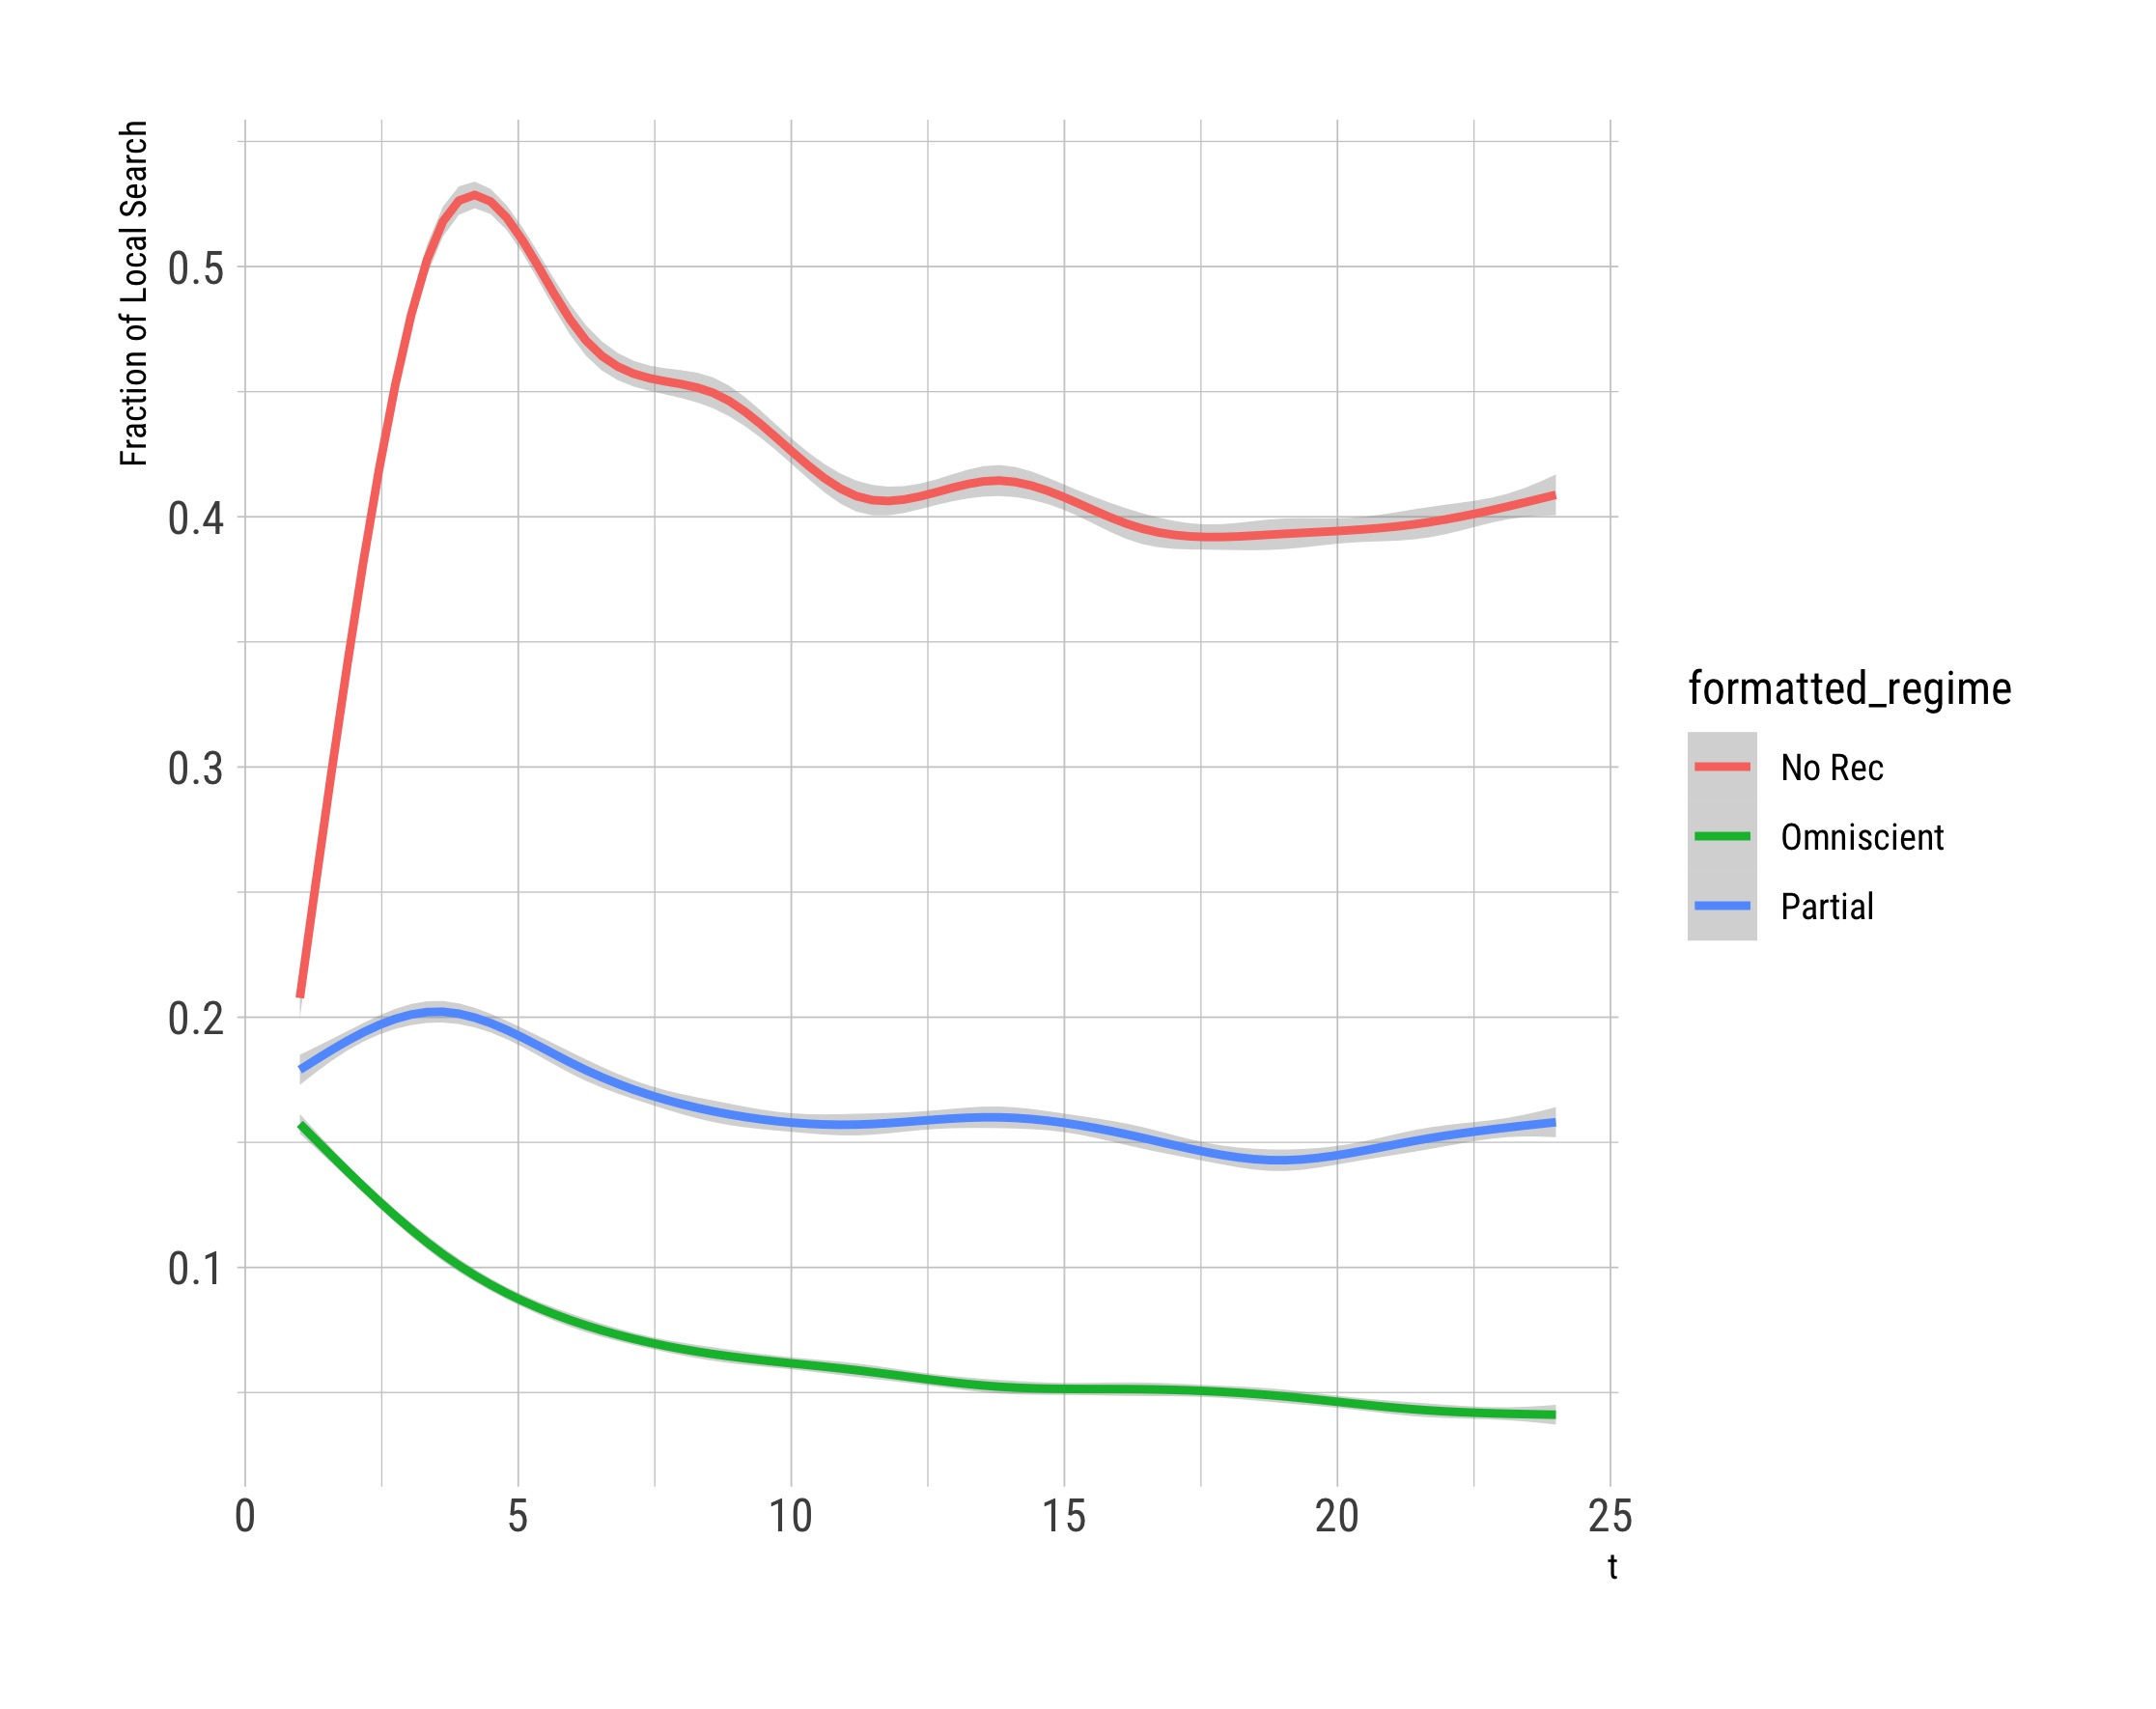
\includegraphics[scale=0.08]{figures/local_moves_25}
\caption{Fraction of users who engage in ``local" consumption - moving less than 10 units}
\label{fig:local_consumption}
\end{figure}

\begin{figure}
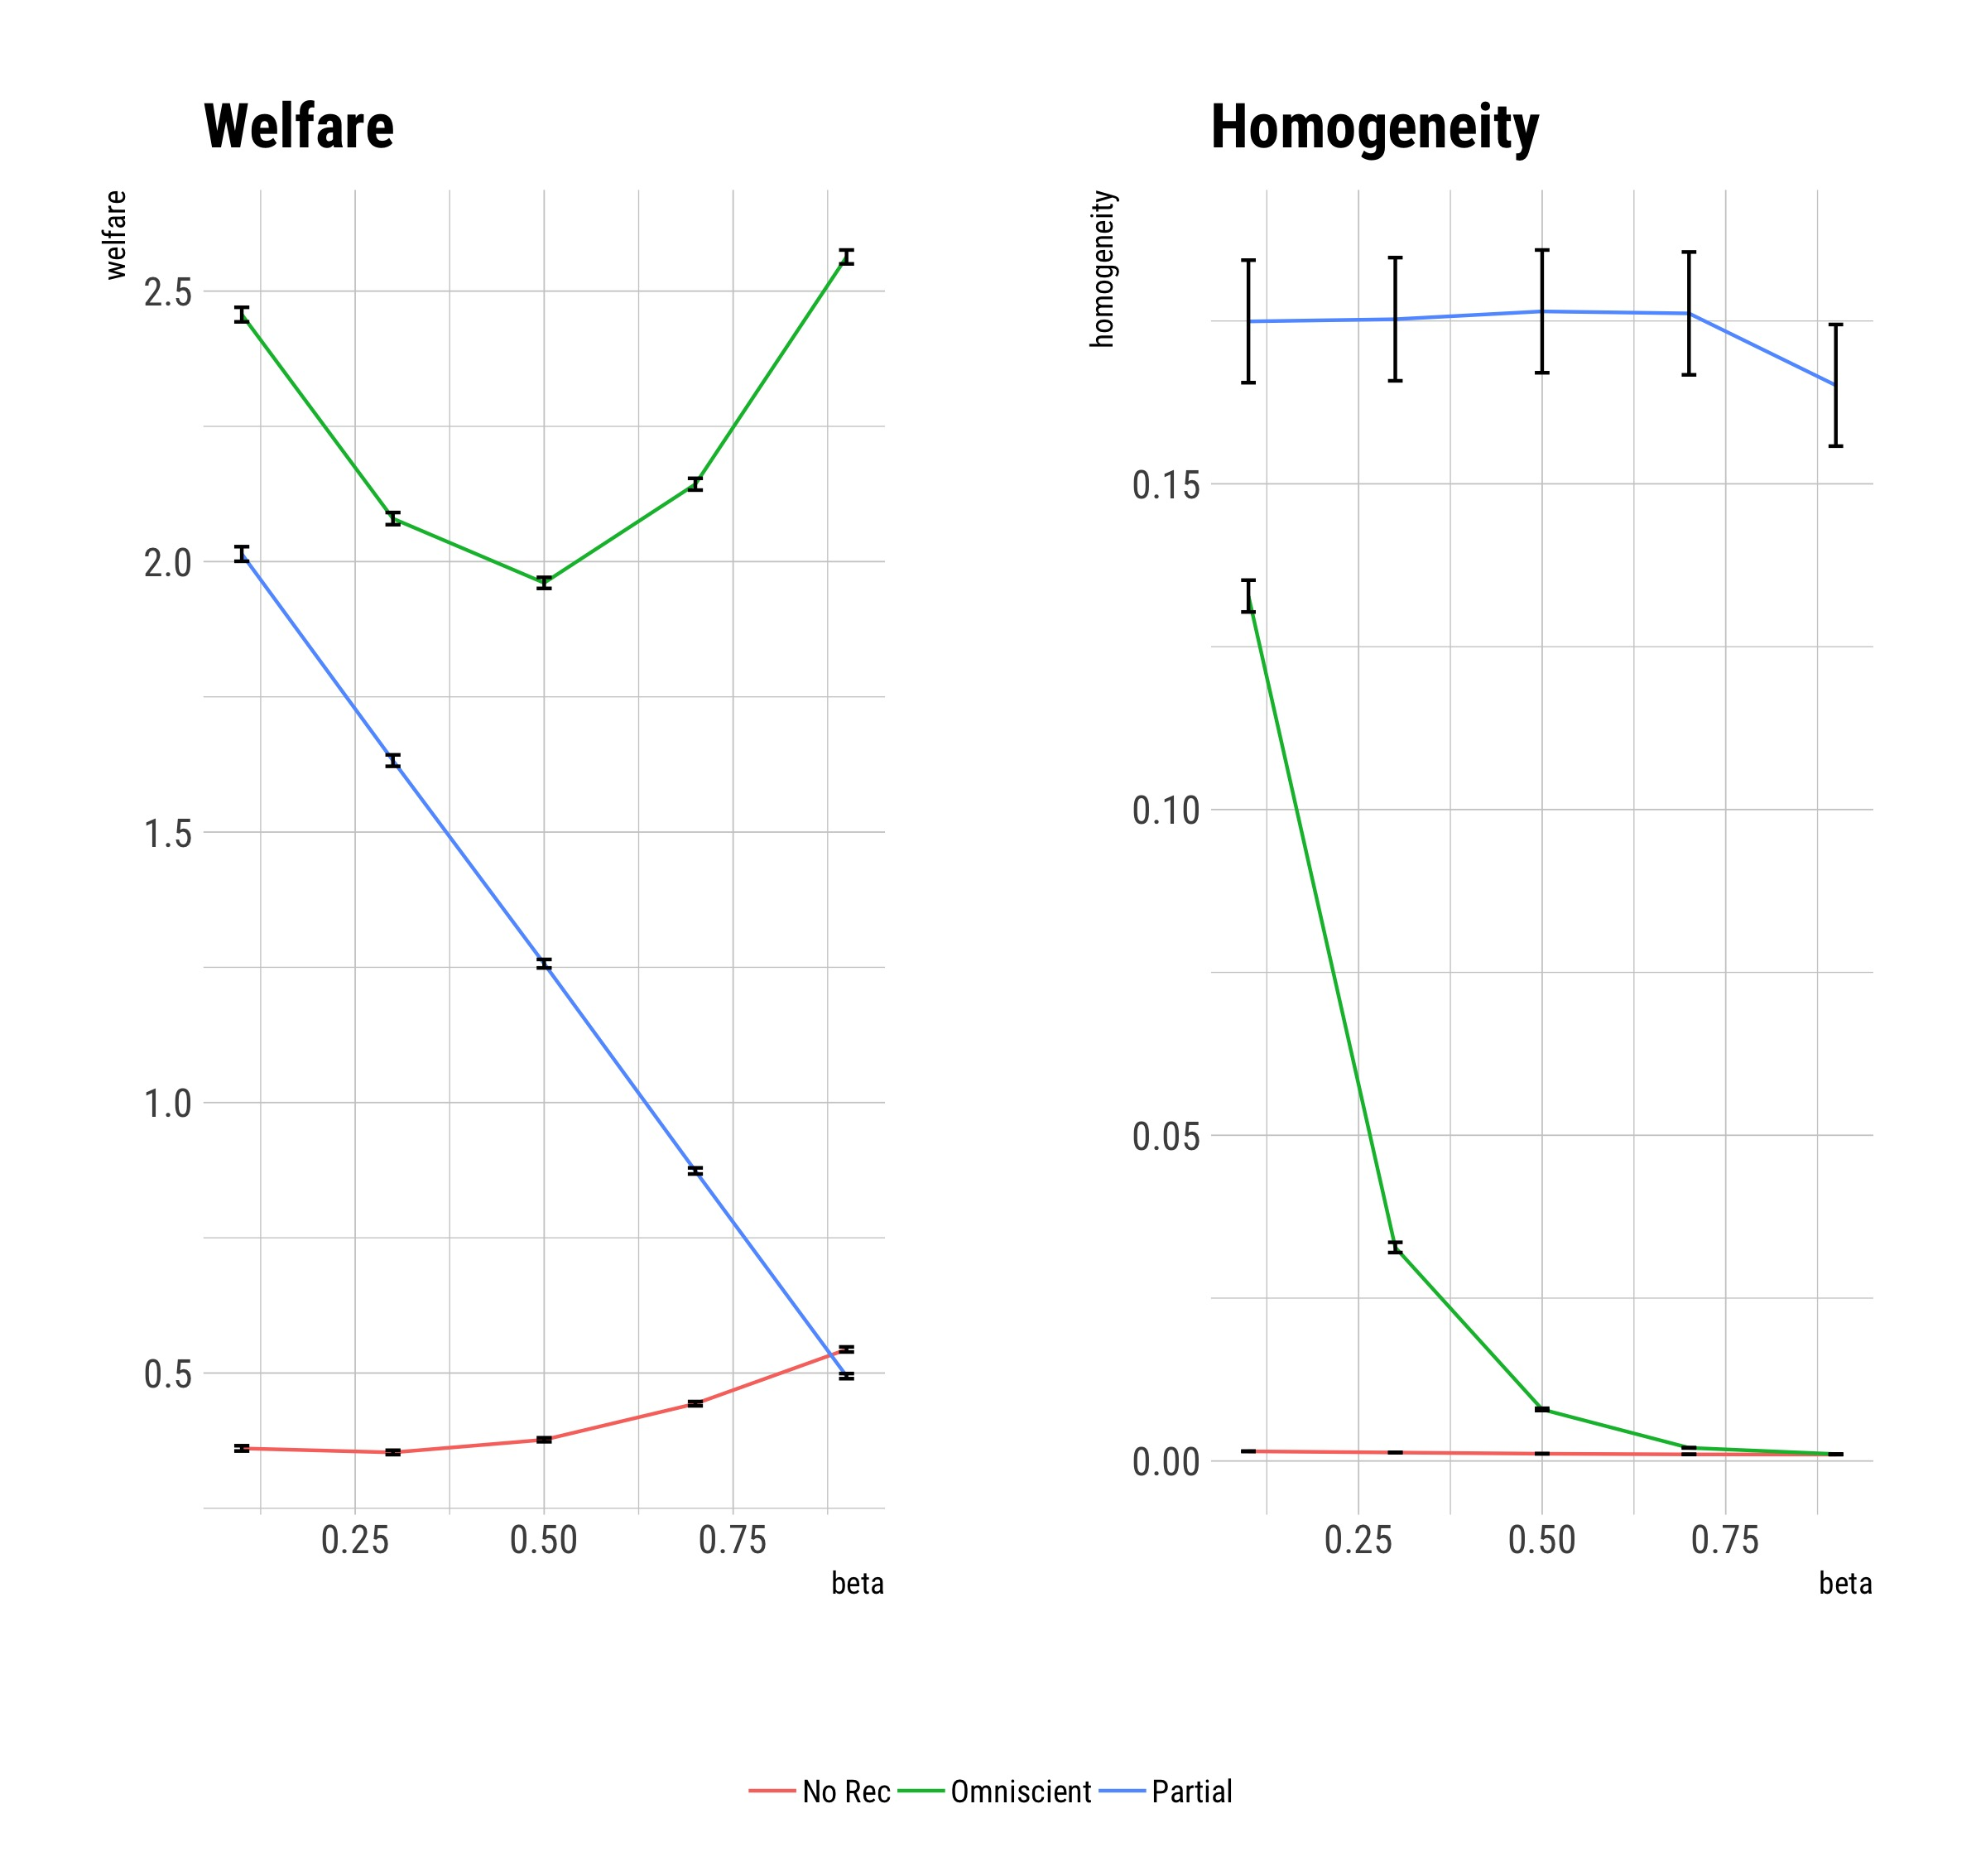
\includegraphics[scale=0.05]{figures/welfare_homo_combo}
\caption{Welfare and Homogeneity varying $\beta$}
\label{fig:beta_vary}
\end{figure}
\par
Furthermore, \cite{nguyen2014exploring} also find that recommendation can lead to an increase in consumption diversity. As Table \ref{table:agg_results} shows, our model is consistent with this effect but it depends on the nature of recommendation. If recommendation only provides information on the common-value component then welfare and consumption diversity increase but, correspondingly, homogenization increases dramatically. If recommendation takes into account user beliefs on the idiosyncratic  component of utility then welfare and consumption diversity can further increase and homogeneity will decrease.
\par
Low consumption diversity by itself is not necessarily bad. Figure \ref{fig:diversity_welfare_no_rec} shows that in the no recommendation case welfare and consumption diversity are negatively correlated. This is primarily because content diversity in the no recommendation case can arise from the fact that the user consumes a bad product and is forced to jump around the product space looking for ``good " products. However, if a user finds a high utility product right away then staying in this neighborhood may yield higher utility due to the correlation of utilities. The problem is that, even when the user finds a ``good" product, this may only be ``locally" good and the user will then excessively consume goods around it.
\par
As users learn more about the idiosyncratic component of their own preferences (i.e. as $t$ increases), the value of recommendation decreases. Figure \ref{fig:rec_obey} shows that recommendation compliance decreases as $t$ increases. Additionally, Figure \ref{fig:fig:beta_vary} shows how homogeneity and welfare change as $\beta$ increases  Most interestingly, when $\beta$ is high recommendation can be harmful to users - user homogeneity remains similar as $\beta$ increases but welfare drops to be even lower than under no recommendation.


\begin{figure}
   \begin{minipage}{0.48\textwidth}
     \centering
     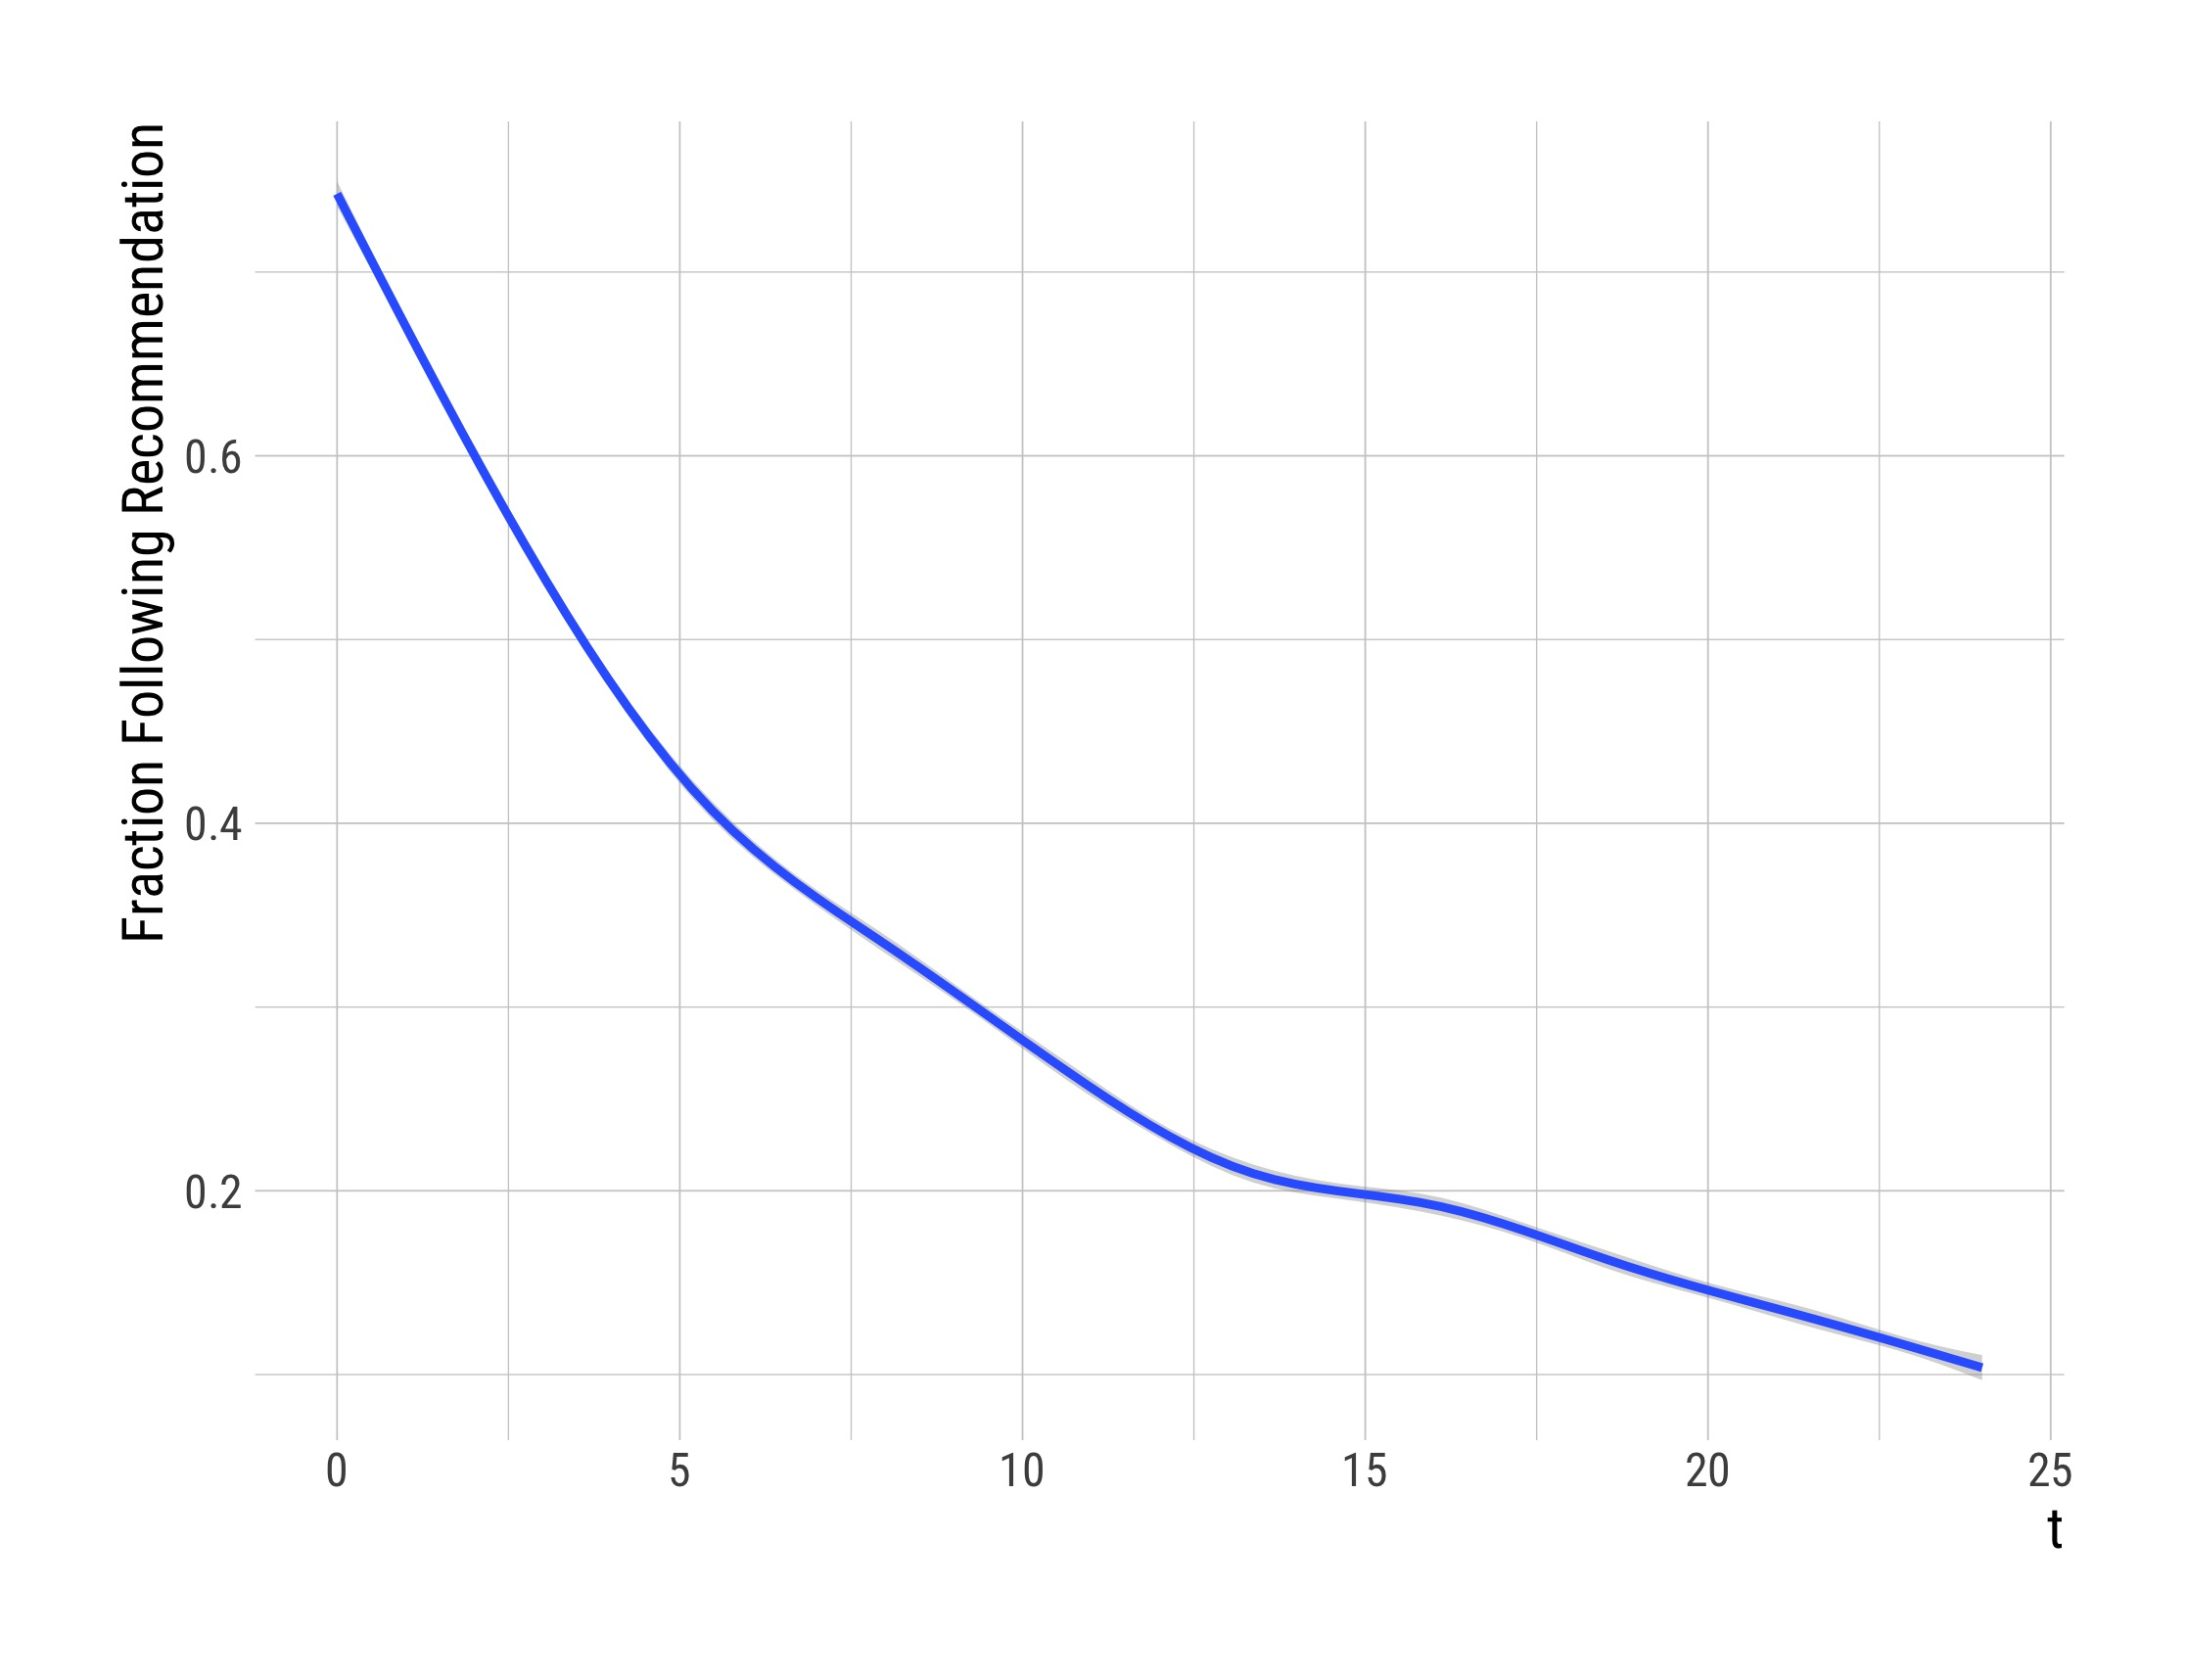
\includegraphics[width=.5\linewidth]{figures/rec_obedience_25}
     \caption{Recommendation Effectiveness}\label{fig:rec_obey}
   \end{minipage}\hfill
   \begin{minipage}{0.48\textwidth}
     \centering
     \includegraphics[width=.5\linewidth]{"figures/Diversity vs Welfare - No Recommendation"}
     \caption{Diversity vs Welfare under No Recommendation}\label{fig:diversity_welfare_no_rec}
   \end{minipage}
\end{figure}

\section{Conclusion}

We have argued that incorporating user choice under uncertainty should be a first-order component of RS design. By collecting appropriate data about user choices and user beliefs, RS can be built to better understand what choices users are likely to make and thus what information would be useful to give them as opposed to simply predicting what items a user will like. This approach can not only aid in designing more useful RS, but can also be utilized to better understand recently documented adverse effects of RS such as filter bubbles and homogenization. We presented a model of user choice under uncertainty with correlated utilities that naturally generates filter bubble effects without any recommendation. We showed how, by not properly incorporating user beliefs into recommendation, RS can help alleviate filter bubble effects and increase utility but also substantially increase homogenization amongst users. Incorporating user beliefs can help increase utility even further but decrease homogenization effects. We leave for future work approaches that incorporate the insights from our work into traditional recommender system design methods.

\bibliographystyle{plain}
\bibliography{refs}
\end{document}
